\section{Identification of Associations}

Associations link entities together. We identify associations from subject-verb-object sentences in the specifications. The verb represents the association between two entities (Subject, Object).

\subsection{Entity-Association}
Based on the Union Cycliste Internationale specifications, we extract key sentences that connect entities through verbs:

\begin{itemize}
\item A person \textbf{is} a rider.
\item A person \textbf{is} a sports director.
\item A person \textbf{is} a soigneur.
\item A rider \textbf{belongs to} a team.
\item A soigneur \textbf{treats} a rider.
\item A stage \textbf{is won by} a rider.
\item A ranking \textbf{determines the position of} a rider.
\item A ranking \textbf{is achieved during} a stage.
\item A race \textbf{includes} stages.
\item A stage \textbf{is won by} a team.
\item A soigneur \textbf{provides treatment during} a race.
\item A soigneur \textbf{treats at the request of} a team.
\end{itemize}

\subsection{UML Modeling (Version 1.1)}
From these associations between entities, we can propose an initial version of the database structure using UML formalism.

\begin{figure}[H]
\begin{center}
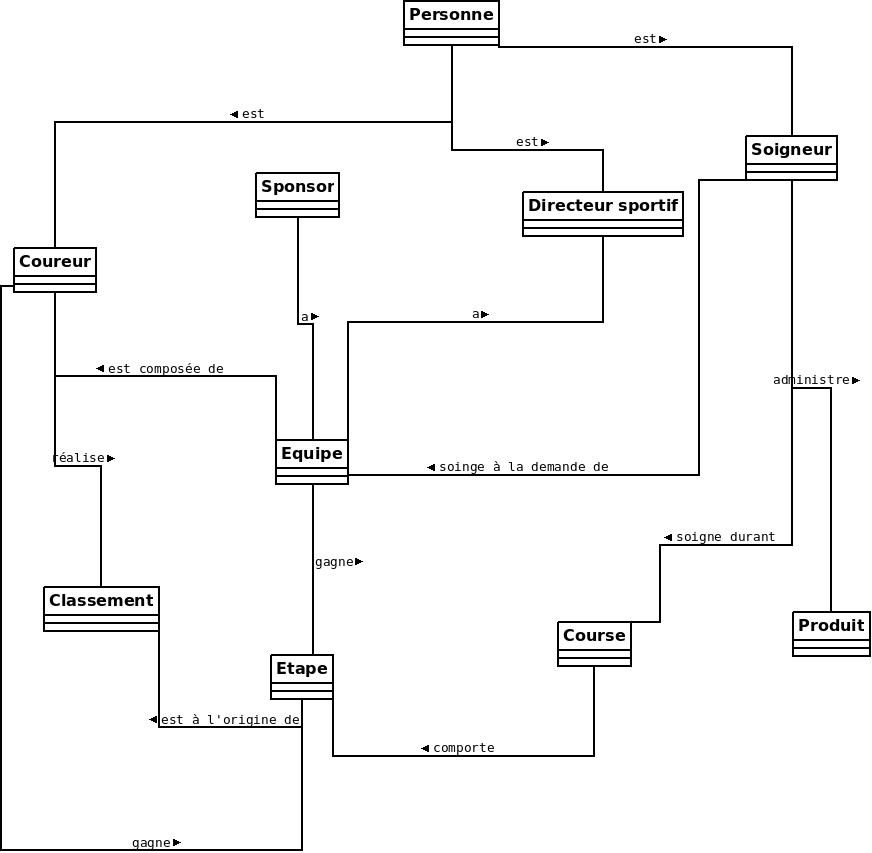
\includegraphics[height=7cm]{Figure1.jpg}\\
\caption{Model: Entity-Association}
\label{fig1}
\end{center}
\end{figure}
